\chapter{Hypothetical Home}\label{ch:hypothetical_home}

An hypothethical home was designed as a starting point for the creation of the \acrshort{dt}. A number of appliance types were chosen to be introduced into the home, based on their commonality in European households and their availability in the GREEND and UK-DALE datasets. These two datasets were selected among the ones studied (see Chapter~\ref{ch:analysis_of_smart_home_datasets}) because they provide a large number of appliances, and they contain data about European households. This is significant in order to minimize the geographic variations in appliance usage patterns and to produce results that can be relevant for Italian households. The floor plan of the home is shown in Figure~\ref{fig:home_floor_plan}, showing the location of the following chosen appliances:
\begin{itemize}
  \item a fridge with combined freezer;
  \item a washing machine;
  \item a dishwasher;
  \item a radio;
  \item two TVs;
  \item a desktop computer;
  \item six lamps;
  \item a microwave;
  \item three \acrshort{ac} splits;
  \item a boiler.
\end{itemize}

\begin{figure}
  \centering
  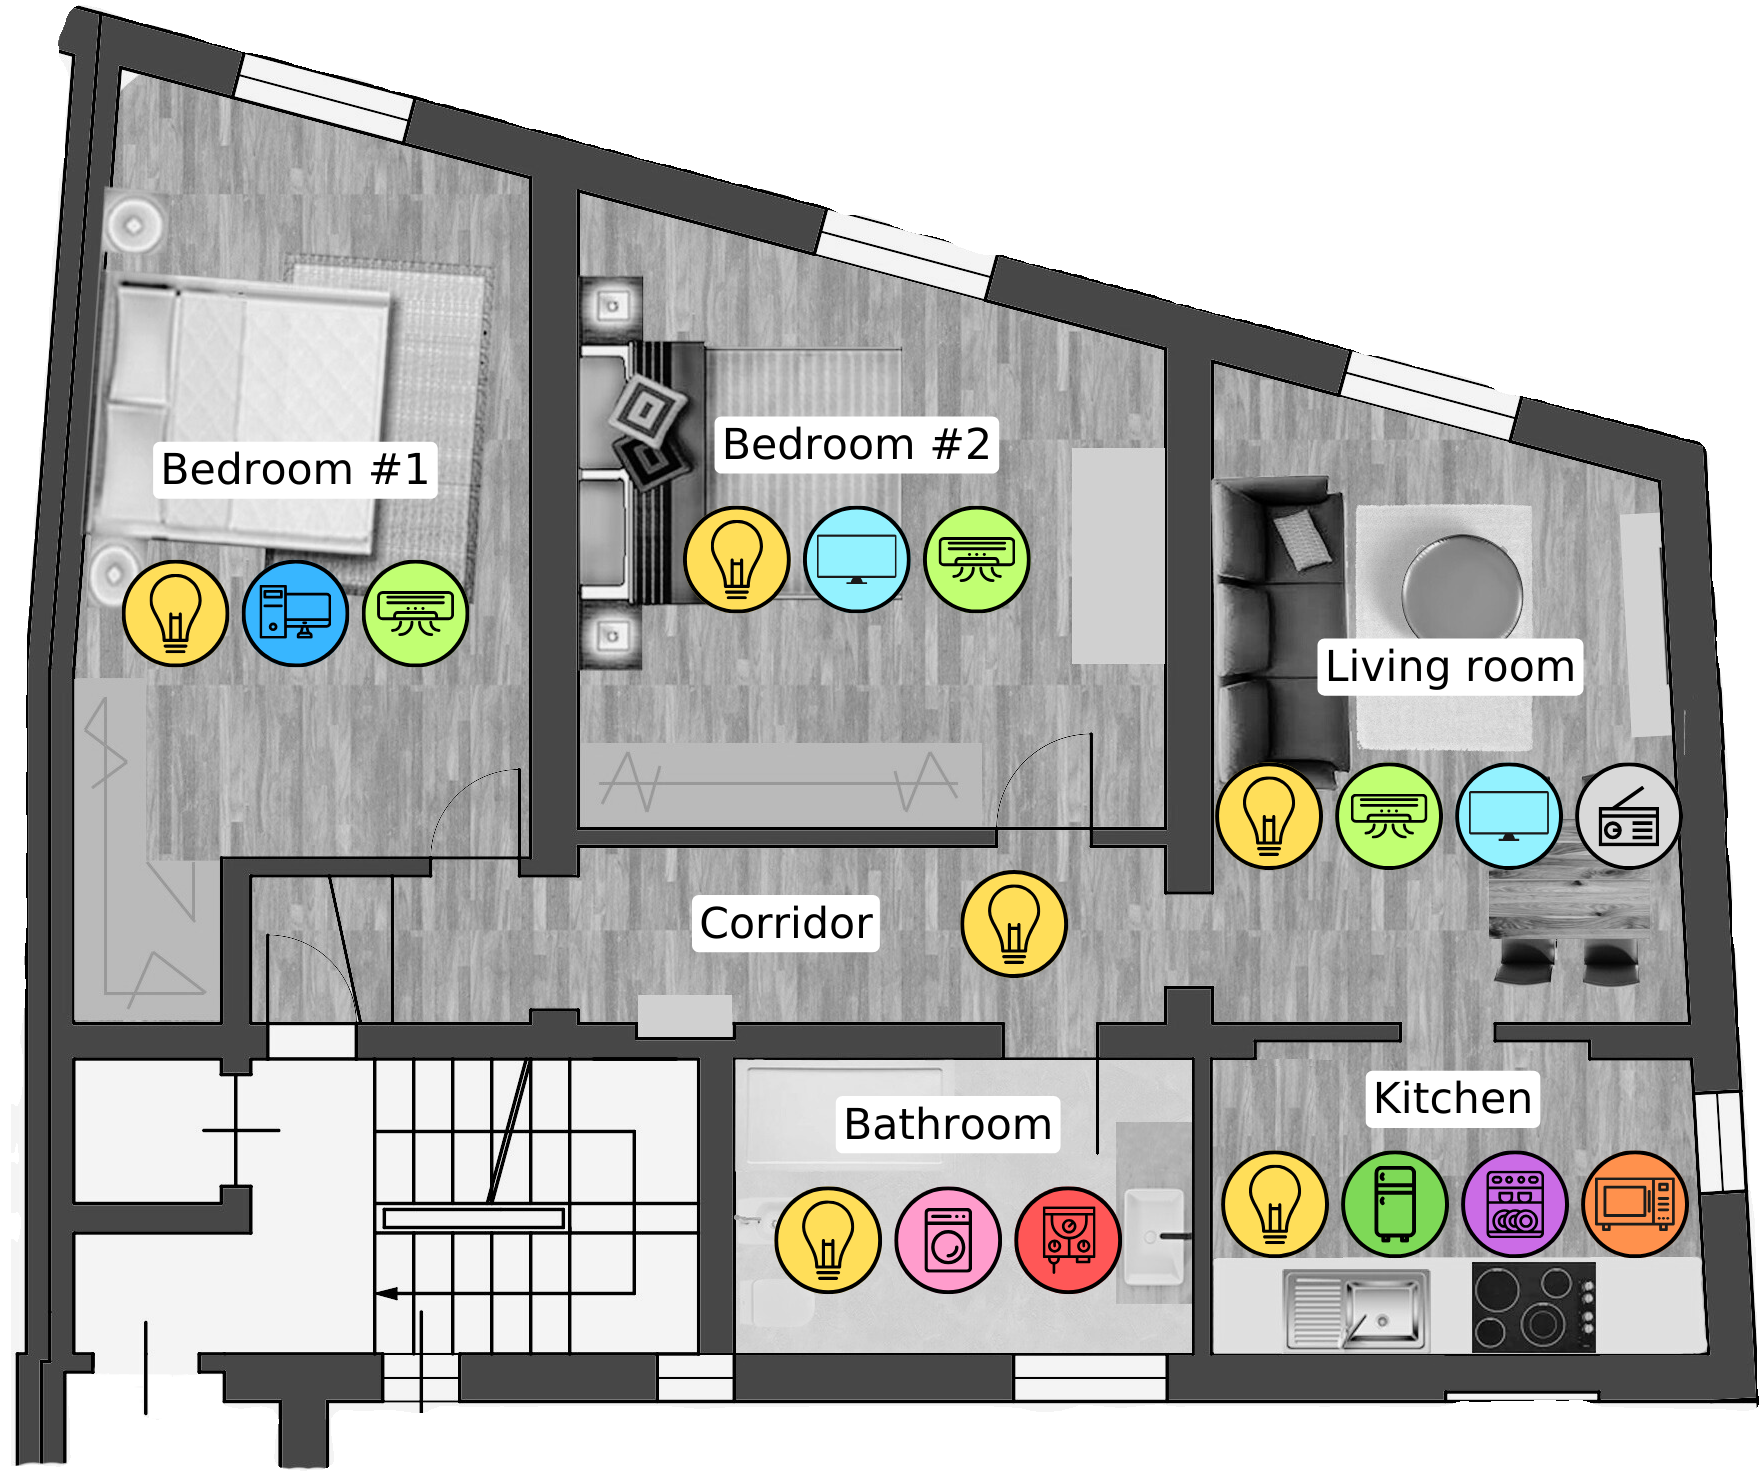
\includegraphics[width=0.75\linewidth]{images/floor_plan.png}
  \caption{Floor plan of a hypothetical case study home with the location of the chosen appliance types.}
  \label{fig:home_floor_plan}
\end{figure}

For each appliance type, a specific appliance studied in one of the buildings in GREEND or UK-DALE was chosen as a representative sample. Table~\ref{tab:appliances_details} shows the details of the selected appliances, including the source dataset, the building, the manufacturer, and the model. The preferred sources were the buildings $3$ and $5$ of the GREEND dataset, as they had a large number of appliance data and reasonable consumption values. Other buildings in GREEND were discarded, as they either contained insufficient usage data, or the consumptions were highly unrealistic, indicating measurement errors. The appliance types that were either unavailable or unsuitable in GREEND were instead chosen from the UK-DALE dataset. Again, the buildings and appliances were chosen with the same criteria as GREEND. Because no information about individual \acrshort{ac} splits was available, the whole-home \acrshort{ac} consumption was used instead. This corresponds to the three splits being controlled collectively.

\begin{table}
  \centering
  \begin{tabular}{llcll}
    \hline
    \textbf{Appliance type} & \textbf{Dataset} & \textbf{Building} & \textbf{Manufacturer} & \textbf{Model} \\ \hline
    Radio                   & GREEND           & 3                 & Denon                 & DRA-275RD      \\
    Dishwasher              & GREEND           & 5                 & Whirlpool             & ADG 555 IX     \\
    Fridge w/ freezer       & GREEND           & 5                 & Siemens               &                \\
    Television              & GREEND           & 5                 & Samsung               & LE32C650       \\
    Microwave               & GREEND           & 3                 & Whirlpool             & AMW 494/IX     \\
    Lamp                    & UK-DALE          & 1                 &                       &                \\
    Washing machine         & GREEND           & 3                 & Zanussi               & F1215          \\
    Desktop                 & GREEND           & 5                 & Dimotion              & QuietONE Q2    \\
    Boiler                  & UK-DALE          & 4                 &                       &                \\
    AC                      & UK-DALE          & 5                 &                       &                \\ \hline
  \end{tabular}%
  \caption{Details of selected appliances. Missing cells indicate that the information is not provided.}
  \label{tab:appliances_details}
\end{table}

A limitation of both the GREEND an UK-DALE datasets is that they do not record the operation mode of appliances at a given time. This information is required in order to assign a specific consumption value to the operation modes, and to estimate their duration. The other datasets introduced in Chapter~\ref{ch:analysis_of_smart_home_datasets} that do provide this type of information are either too imprecise about the start/end time or limited in the number of appliances they record.

A possible solution is identifying the operation mode of appliances from the power consumption data using unsupervised learning methods. A naive approach to doing so is clustering the raw energy values: this can work for simple appliances, such as lamps or televisions, but not for complex ones with \textit{operation cycles}, such as fridges or washing machines. For example, a washing machine might draw no power for a short period while the clothes soak, and then use a lot of power for a spin cycle. Both of these cycles are part of the same operation mode, but there is no way to recognize this when clustering the raw data. Furthermore, methods based on raw data are also susceptible to noisy points and outliers; thus, they often lead to poor clustering results~\parencite{castangiaClusteringApplianceOperation2023}.

The approach used in this thesis is inspired by the one proposed by~\cite{castangiaClusteringApplianceOperation2023}, which uses unsupervised deep learning techniques to cluster appliance operation modes from a learned, \textit{latent state} representation of the raw data. Figure~\ref{fig:high_level_procedure} illustrates the main steps of the approach. First, a segmentation procedure is applied to the raw appliance data to identify the active states that contain the actual power signatures of the device. These signatures are then standardized and fed to a deep autoencoder model, which learns to reconstruct the operation cycles and to encode them into a latent representation. Next, a K-means clustering algorithm is applied to the latent representation, which groups the operation cycles into different programs of the device. Finally, the clusters are mapped to operation modes of the appliance. The remaining sections in this chapter describe the steps in more detail. The code for the extraction of activations is available on GitHub\footnote{\url{https://github.com/LucaCtt/appliances_data_extraction}}, while the remaining steps are executed in a Google Colab notebook\footnote{\url{https://colab.research.google.com/drive/1blnoyyP10gGdRL6b4JzaeBLg8zs2kVv9?usp=sharing}}.

\begin{figure}
  \centering
  
\includegraphics[width=\linewidth]{images/modes_clustering/high_level_procedure.png}
  \caption{High level procedure for identifying the operation modes of appliances.}
  \label{fig:high_level_procedure}
\end{figure}

\section{Extraction of Appliances Activations}

An \textit{appliance activation} is defined as a sequence of power consumption values gathered in a time interval in which the appliance is switched on. An example of an activation for the fridge in building 3 of GREEND is reported in Listing~\ref{lst:activation_example}, which highlights how the consumption values change during the activation. The goal of extracting the activations is to identify the distinct operations of an appliance based on the continuous active power measurements available, which however include time intervals in which the appliances are switched off, and can thus be filtered out. The power consumption when an appliance is off is assumed to be zero.

To identify the activations, the GREEN and UK-DALE datasets were accessed using NILMTK\footnote{\url{https://github.com/nilmtk/nilmtk}}, a Python toolkit designed for comparing the performance of energy disaggregation algorithms~\parencite{batraItDifferentInsights2013}, which also provides data analysis functions for NILM datasets. The appliance activations were extracted at the default frequency of the datasets (every second for GREEND and every six seconds for UK-DALE) using NILMTK's \texttt{Electric.get\_activations()} method, with three arguments used for configuration:
\begin{itemize}
  \item \texttt{on\_power\_threshold}: the minimum power consumption value (in watts) for the appliance to be considered switched on.
  \item \texttt{min\_off\_duration}: the minimum duration (in seconds) for the appliance to be below \texttt{on\_power\_threshold} to be considered turned off.
  \item \texttt{min\_on\_duration}: the minimum duration (in seconds) for the activation to be valid. This, along with \texttt{min\_off\_duration}, helps to filter out spurious power spikes.
\end{itemize}
The values of these parameters were selected empirically for each appliance, by selecting combinations that produced a balance between the number of activations and their mean length. For example, considering the microwave in building 3 of GREEND, using $\texttt{on\_power\_threshold} = 20$, $\texttt{min\_off\_duration} = 20$, and $\texttt{min\_on\_duration} = 10$ resulted in $2311$ activations, with a mean duration of around $471$ seconds. When using instead $\texttt{on\_power\_threshold} = 10$, $\texttt{min\_off\_duration} = 5$, and $\texttt{min\_on\_duration} = 5$ resulted in $15609$ activations, with a mean duration close however to just $78$ seconds.

\newpage

The sampling frequency of the activations is the default one provided by the datasets, which correspond to $1$ second for GREEND and $6$ seconds UK-DALE. The resulting activations were then clipped to a maximum threshold to eliminate noise. The maximum thresholds were chosen using the plots of the raw power consumption data of each appliance, represented in Figures~\ref{fig:raw_power_consumptions_greend} and~\ref{fig:raw_power_consumptions_uk_dale}, by selecting values that remove spurious power spikes. It can be observed from Figure~\ref{fig:ac} that the consumptions of the AC are unrealistically high. Due to the lack of other AC appliances in the datasets, the data was clipped and used anyway. Table~\ref{tab:activation_details} shows the parameters and the number of activations obtained for each appliance type.

\begin{lstlisting}[language=plain,caption={[Example of an activation]Example of an activation for the fridge in building 3 of the GREEND dataset. The numbers are samples of the energy consumption (in watts) gathered every second.},label=lst:activation_example,float,floatplacement=H]
0.000000 0.000000 66.601420 120.160070 63.387650 63.387650 173.715010 175.85713 130.871350 10.896457 ... 177.99924 186.56764 186.56764 188.70972 186.56764 201.56210 207.98820 201.56210 207.98820
\end{lstlisting}

\begin{figure}
  \begin{subfigure}{.5\textwidth}
    \centering
    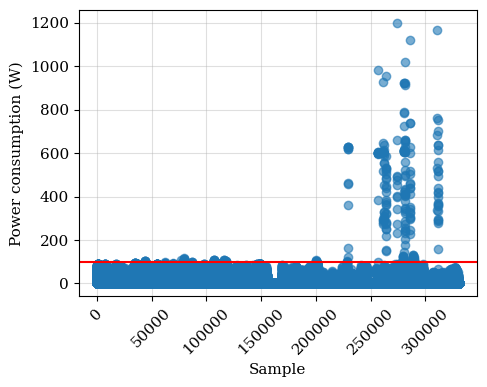
\includegraphics[width=.9\linewidth]{images/raw_consumptions/audio_amplifier.png}
    \caption{Radio}
    \label{fig:radio}
  \end{subfigure}%
  \begin{subfigure}{.5\textwidth}
    \centering
    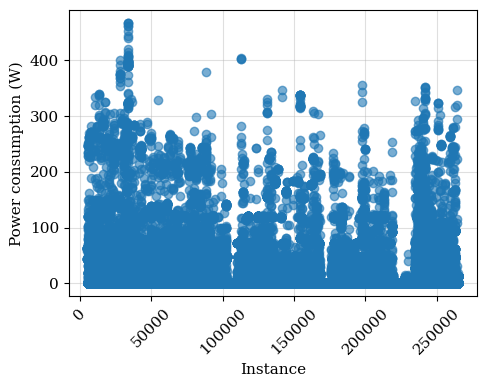
\includegraphics[width=.9\linewidth]{images/raw_consumptions/dish_washer.png}
    \caption{Dishwasher}
    \label{fig:dish_washer}
  \end{subfigure}
  \begin{subfigure}{.5\textwidth}
    \centering
    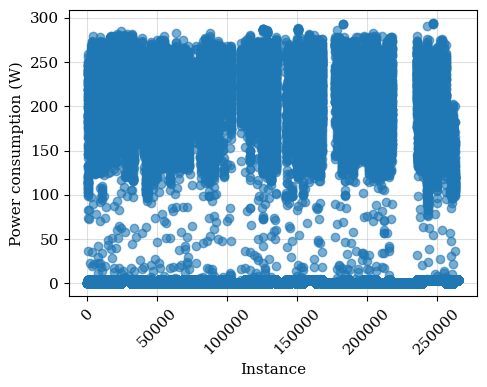
\includegraphics[width=.9\linewidth]{images/raw_consumptions/fridge.png}
    \caption{Fridge freezer}
    \label{fig:fridge_freezer}
  \end{subfigure}%
  \begin{subfigure}{.5\textwidth}
    \centering
    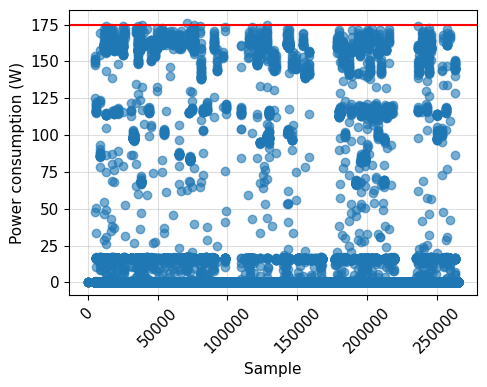
\includegraphics[width=.9\linewidth]{images/raw_consumptions/television.png}
    \caption{Television}
    \label{fig:television}
  \end{subfigure}
  \begin{subfigure}{.5\textwidth}
    \centering
    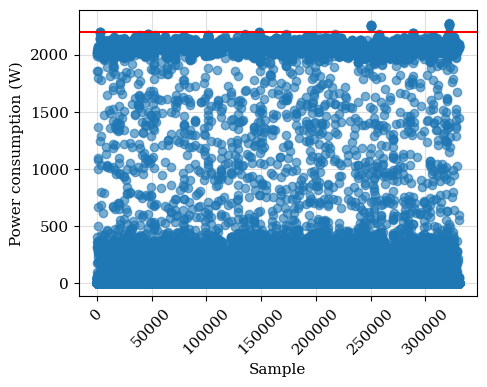
\includegraphics[width=.9\linewidth]{images/raw_consumptions/microwave.png}
    \caption{Microwave}
    \label{fig:microwave}
  \end{subfigure}%
  \begin{subfigure}{.5\textwidth}
    \centering
    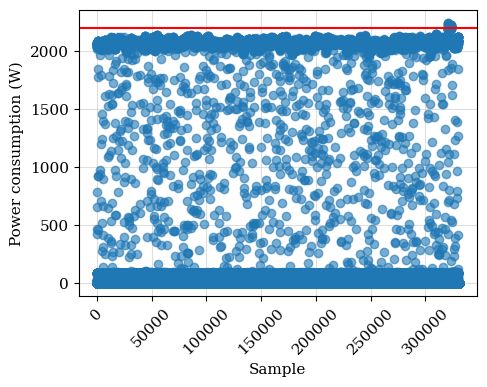
\includegraphics[width=.9\linewidth]{images/raw_consumptions/washing_machine.png}
    \caption{Washing machine}
    \label{fig:washing_machine}
  \end{subfigure}
\end{figure}%
\begin{figure}\ContinuedFloat
  \begin{subfigure}{\textwidth}
    \centering
    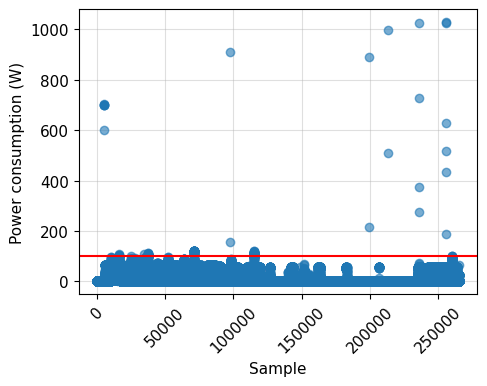
\includegraphics[width=.45\linewidth]{images/raw_consumptions/desktop_computer.png}
    \caption{Desktop computer}
    \label{fig:desktop_computer}
  \end{subfigure}
  \caption[Raw power consumptions of appliances extracted from GREEND]{Raw power consumptions of appliances extracted from GREEND. The samples are gathered every second. The red line represents the maximum threshold used to clip the activations.}
  \label{fig:raw_power_consumptions_greend}
\end{figure}

\begin{figure}
  \begin{subfigure}{.5\textwidth}
    \centering
    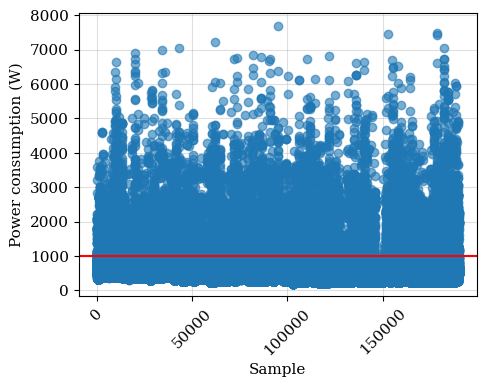
\includegraphics[width=.9\linewidth]{images/raw_consumptions/ac.png}
    \caption{AC}
    \label{fig:ac}
  \end{subfigure}%
  \begin{subfigure}{.5\textwidth}
    \centering
    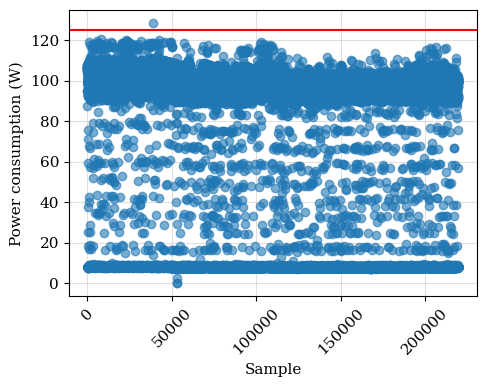
\includegraphics[width=.9\linewidth]{images/raw_consumptions/boiler.png}
    \caption{Boiler}
    \label{fig:boiler}
  \end{subfigure}
  \begin{subfigure}{\textwidth}
    \centering
    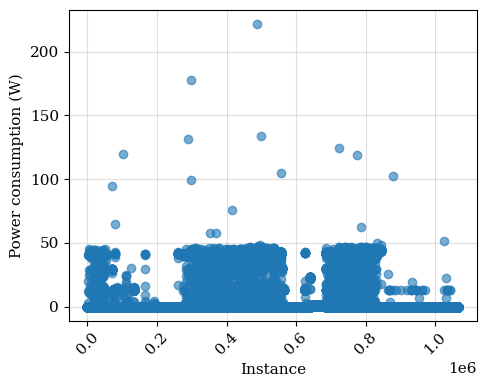
\includegraphics[width=.42\linewidth]{images/raw_consumptions/lamp.png}
    \caption{Lamp}
    \label{fig:lamp}
  \end{subfigure}
  \caption[Raw power consumptions of appliances extracted from UK-DALE]{Raw power consumptions of appliances extracted from UK-DALE. The samples are gathered every six seconds. The red line represents the maximum threshold used to clip the activations.}
  \label{fig:raw_power_consumptions_uk_dale}
\end{figure}

\begin{table}
  \centering
  \resizebox{\textwidth}{!}{%
    \begin{tabular}{lccccc}
      \hline
      \textbf{Appliance type}                               &
      \multicolumn{1}{l}{\textbf{Min on (s)}}               &
      \multicolumn{1}{l}{\textbf{Min off (s)}}              &
      \multicolumn{1}{l}{\textbf{Activation Threshold (W)}} &
      \multicolumn{1}{l}{\textbf{Max Threshold (W)}}        &
      \multicolumn{1}{l}{\textbf{\# Activations}}                                           \\ \hline
      Radio                                                 & 5   & 5   & 10  & 100  & 1344 \\
      Dishwasher                                            & 90  & 90  & 30  & 400  & 727  \\
      Fridge w/ freezer                                     & 0   & 30  & 40  & 300  & 237  \\
      Television                                            & 20  & 20  & 10  & 175  & 239  \\
      Microwave                                             & 20  & 10  & 20  & 2200 & 2311 \\
      Lamp                                                  & 1   & 1   & 5   & 50   & 812  \\
      Washing machine                                       & 30  & 30  & 20  & 2200 & 609  \\
      Desktop                                               & 20  & 10  & 10  & 100  & 331  \\
      Boiler                                                & 10  & 5   & 50  & 125  & 607  \\
      AC                                                    & 120 & 120 & 300 & 1000 & 1095 \\ \hline
    \end{tabular}%
  }
  \caption{Activation details for each appliance.}
  \label{tab:activation_details}
\end{table}

\section{Autoencoder}

An autoencoder is a type of neural network capable of learning to compress the inputs into a low-dimensional representation, called the \textit{latent state}, in a totally unsupervised way~\parencite{hintonReducingDimensionalityData2006}. It has two components: an encoder that maps the inputs to the latent state, and a decoder that reconstructs the inputs from the latent state. The goal of the autoencoder is to learn the most relevant features of the inputs by minimizing the difference between the original and the reconstructed inputs, also known as the \textit{reconstruction error}~\parencite{hintonReducingDimensionalityData2006}. An autoencoder can learn the most important features of the activations of an appliance, so that they can be clustered to identify operation modes. Clustering the raw activations is not an effective approach, as it is too susceptible to noise~\parencite{castangiaClusteringApplianceOperation2023}, and requires extensive computational resources due to the high dimensionality of activations. The next sections describe the layers that make up the architecture used in this work.

\subsection{One-dimensional Convolutional Layers}

One-dimensional (1-D) convolutional layers are neural network layers commonly used to process sequential data, such as text, speech, audio, or time series. They learn temporal dependencies and meaningful features from the input data by applying 1-D convolutions~\parencite{kiranyaz1DConvolutionalNeural2021}. A convolution is a mathematical operation that slides a filter or \textit{kernel} over the input and computes the dot product between the filter and the input at each position~\parencite{rudinFunctionalAnalysisTata1973}. 1-D convolutional layers are composed by multiple filters that have the purpose of selecting the most salient features from the input sequence received from the previous layer. The greater the number of filters, the larger the amount of features that can be potentially learned~\parencite{castangiaClusteringApplianceOperation2023}. This is important in order to extract the most significant features of activations, while removing noise. Each filter performs the computation in Equation~\eqref{equ:convolution}, where $n$ is the filter's size, $x_i$ are the inputs, $w_i$ are the filter's weights, $b$ is a bias term, and $f$ is the activation function.
\begin{equation}\label{equ:convolution}
  \tilde{y} = f(\sum_{i=1}^{n}{w_i x_i} + b)
\end{equation}

\newpage

Pooling and upsampling layers often accompany convolutional layers. Pooling layers shrink the output from the convolutional layer. Max pooling does this by taking the maximum value of a sliding window along the input sequence~\parencite{ahmadDeepLearningMultiscale2019}; this helps in selecting the most important features from the input, lower the computation and memory cost, and avoid overfitting~\parencite{zhangDiveDeepLearning2023,masciStackedConvolutionalAutoEncoders2011}. Upsampling layers are somewhat the opposite, as they enlarge their input by inserting zeros between the input values.

\subsection{Long-Short Term Memory}

\acrfull{lstm} is a type of \acrfull{rnn} that can learn long-term dependencies in sequential data. \acrshort{rnn}s are neural networks that have feedback loops, which allow them to process sequential data such as text, speech, audio, or time series~\parencite{ahmadDeepLearningMultiscale2019}. However, \acrshort{rnn}s often suffer from vanishing or exploding gradient, which makes it difficult to learn from distant past inputs or outputs. \acrshort{lstm} solves this problem by introducing a memory cell that can store, update, and retrieve information over long time spans~\parencite{hochreiterLongShortTermMemory1997}. This is useful to learn both the short-term and long-term dependencies among the values of the activations of an appliance.

\acrshort{lstm}s use three gates (input, output, and forget) to control the information flow in and out of the memory cell. These gates can decide what information to keep or discard, based on the current input and the previous state. The full architecture is shown in Figure~\ref{fig:lstm_architecture}. At each time step, the \acrshort{lstm} cell takes the current input $X_t$ and a summary of all previous inputs, which is composed of the short-term state $H_{t-1}$ and the long-term state $C_{t-1}$. Equations~\eqref{equ:lstm_1}---\eqref{equ:lstm_6} show the different operations performed by the \acrshort{lstm} cell, where $W_{xi}$, $W_{xf}$, $W_{xo}$, and $W_{xc}$ are the weights of the input vector $X_t$; $W_{hi}$, $W_{hf}$, $W_{ho}$, and $W_{hc}$ are the weights of the previous short-term state vector $H_{t-1}$; $b_i$, $b_f$, $b_o$, and $b_c$ are the bias terms.
\begin{equation}\label{equ:lstm_1}
  I_t = \sigma(X_{t}W_{xi} + H_{t-1}W_{hi} + b_{i})
\end{equation}
\begin{equation}\label{equ:lstm_2}
  F_t = \sigma(X_{t}W_{xf} + H_{t-1}W_{hf} + b_{f})
\end{equation}
\begin{equation}\label{equ:lstm_4}
  O_t = \sigma(X_{t}W_{xo} + H_{t-1}W_{ho} + b_{o})
\end{equation}
\begin{equation}\label{equ:lstm_3}
  \tilde{C}_t = \tanh(X_{t}W_{xc} + H_{t-1}W_{hc} + b_{c})
\end{equation}
\begin{equation}\label{equ:lstm_5}
  C_t = F_t \odot C_{t-1} + I_t \odot \tilde{C}_t
\end{equation}
\begin{equation}\label{equ:lstm_6}
  H_t = O_t \odot \tanh(C_t)
\end{equation}

\begin{figure}
  \centering
  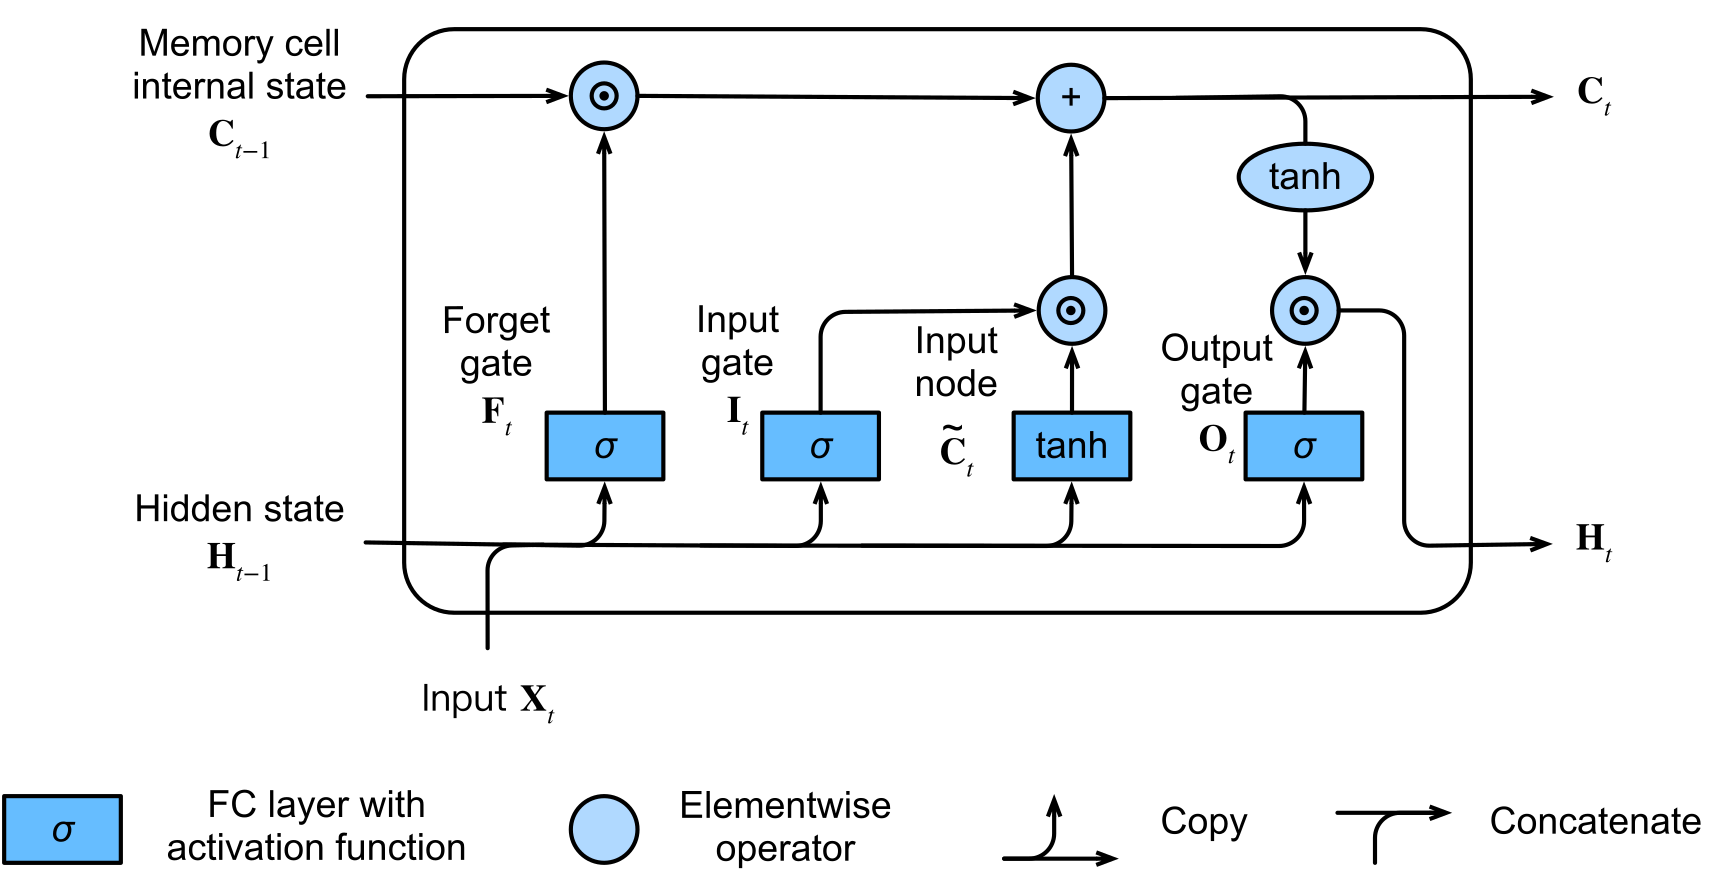
\includegraphics[width=.65\linewidth]{images/modes_clustering/lstm.png}
  \caption[LSTM cell architecture]{LSTM cell architecture. From~\cite{zhangDiveDeepLearning2023}, Subsection 10.1.1, CC-BY-SA license.}
  \label{fig:lstm_architecture}
\end{figure}

A \acrfull{bilstm} is a combination of two \acrshort{lstm}s that process the input sequence in both forward and backward directions~\parencite{schusterBidirectionalRecurrentNeural1997}. One \acrshort{lstm} takes the input sequence as it is, and the other \acrshort{lstm} takes the input sequence in reverse order. The outputs of both \acrshort{lstm}s are then concatenated or summed to produce the final output. A \acrshort{bilstm} can capture both the past and future context of the input sequence and learn which direction is more important for each output step.

\subsection{Autoencoder Architecture and Training}

Figure~\ref{fig:autoencoder_architecture} shows the autoencoder architecture used. The encoder has six convolutional layers with max-pooling layers in between, which halve their input dimensions. It ends with two \acrshort{lstm} layers that capture temporal relations among activation values. The first \acrshort{lstm} layer is bidirectional, and the second is unidirectional. The decoder begins with a repeat vector layer to replicate the latent state six times, in order to reconstruct the correct output dimensions. It then continues with a \acrshort{lstm} layer followed by a series of convolutions and up-sampling layers that double their input dimensions. All convolutional layers have $32$ filters of size $3$, with a \acrfull{relu} activation function. To keep the same sequence length after the convolution, the stride is $1$ and zero padding is added to the input sequence on both sides. The \acrshort{lstm} cells have $128$ units and use a hyperbolic tangent (tanh) activation function.

\begin{figure}
  \centering
  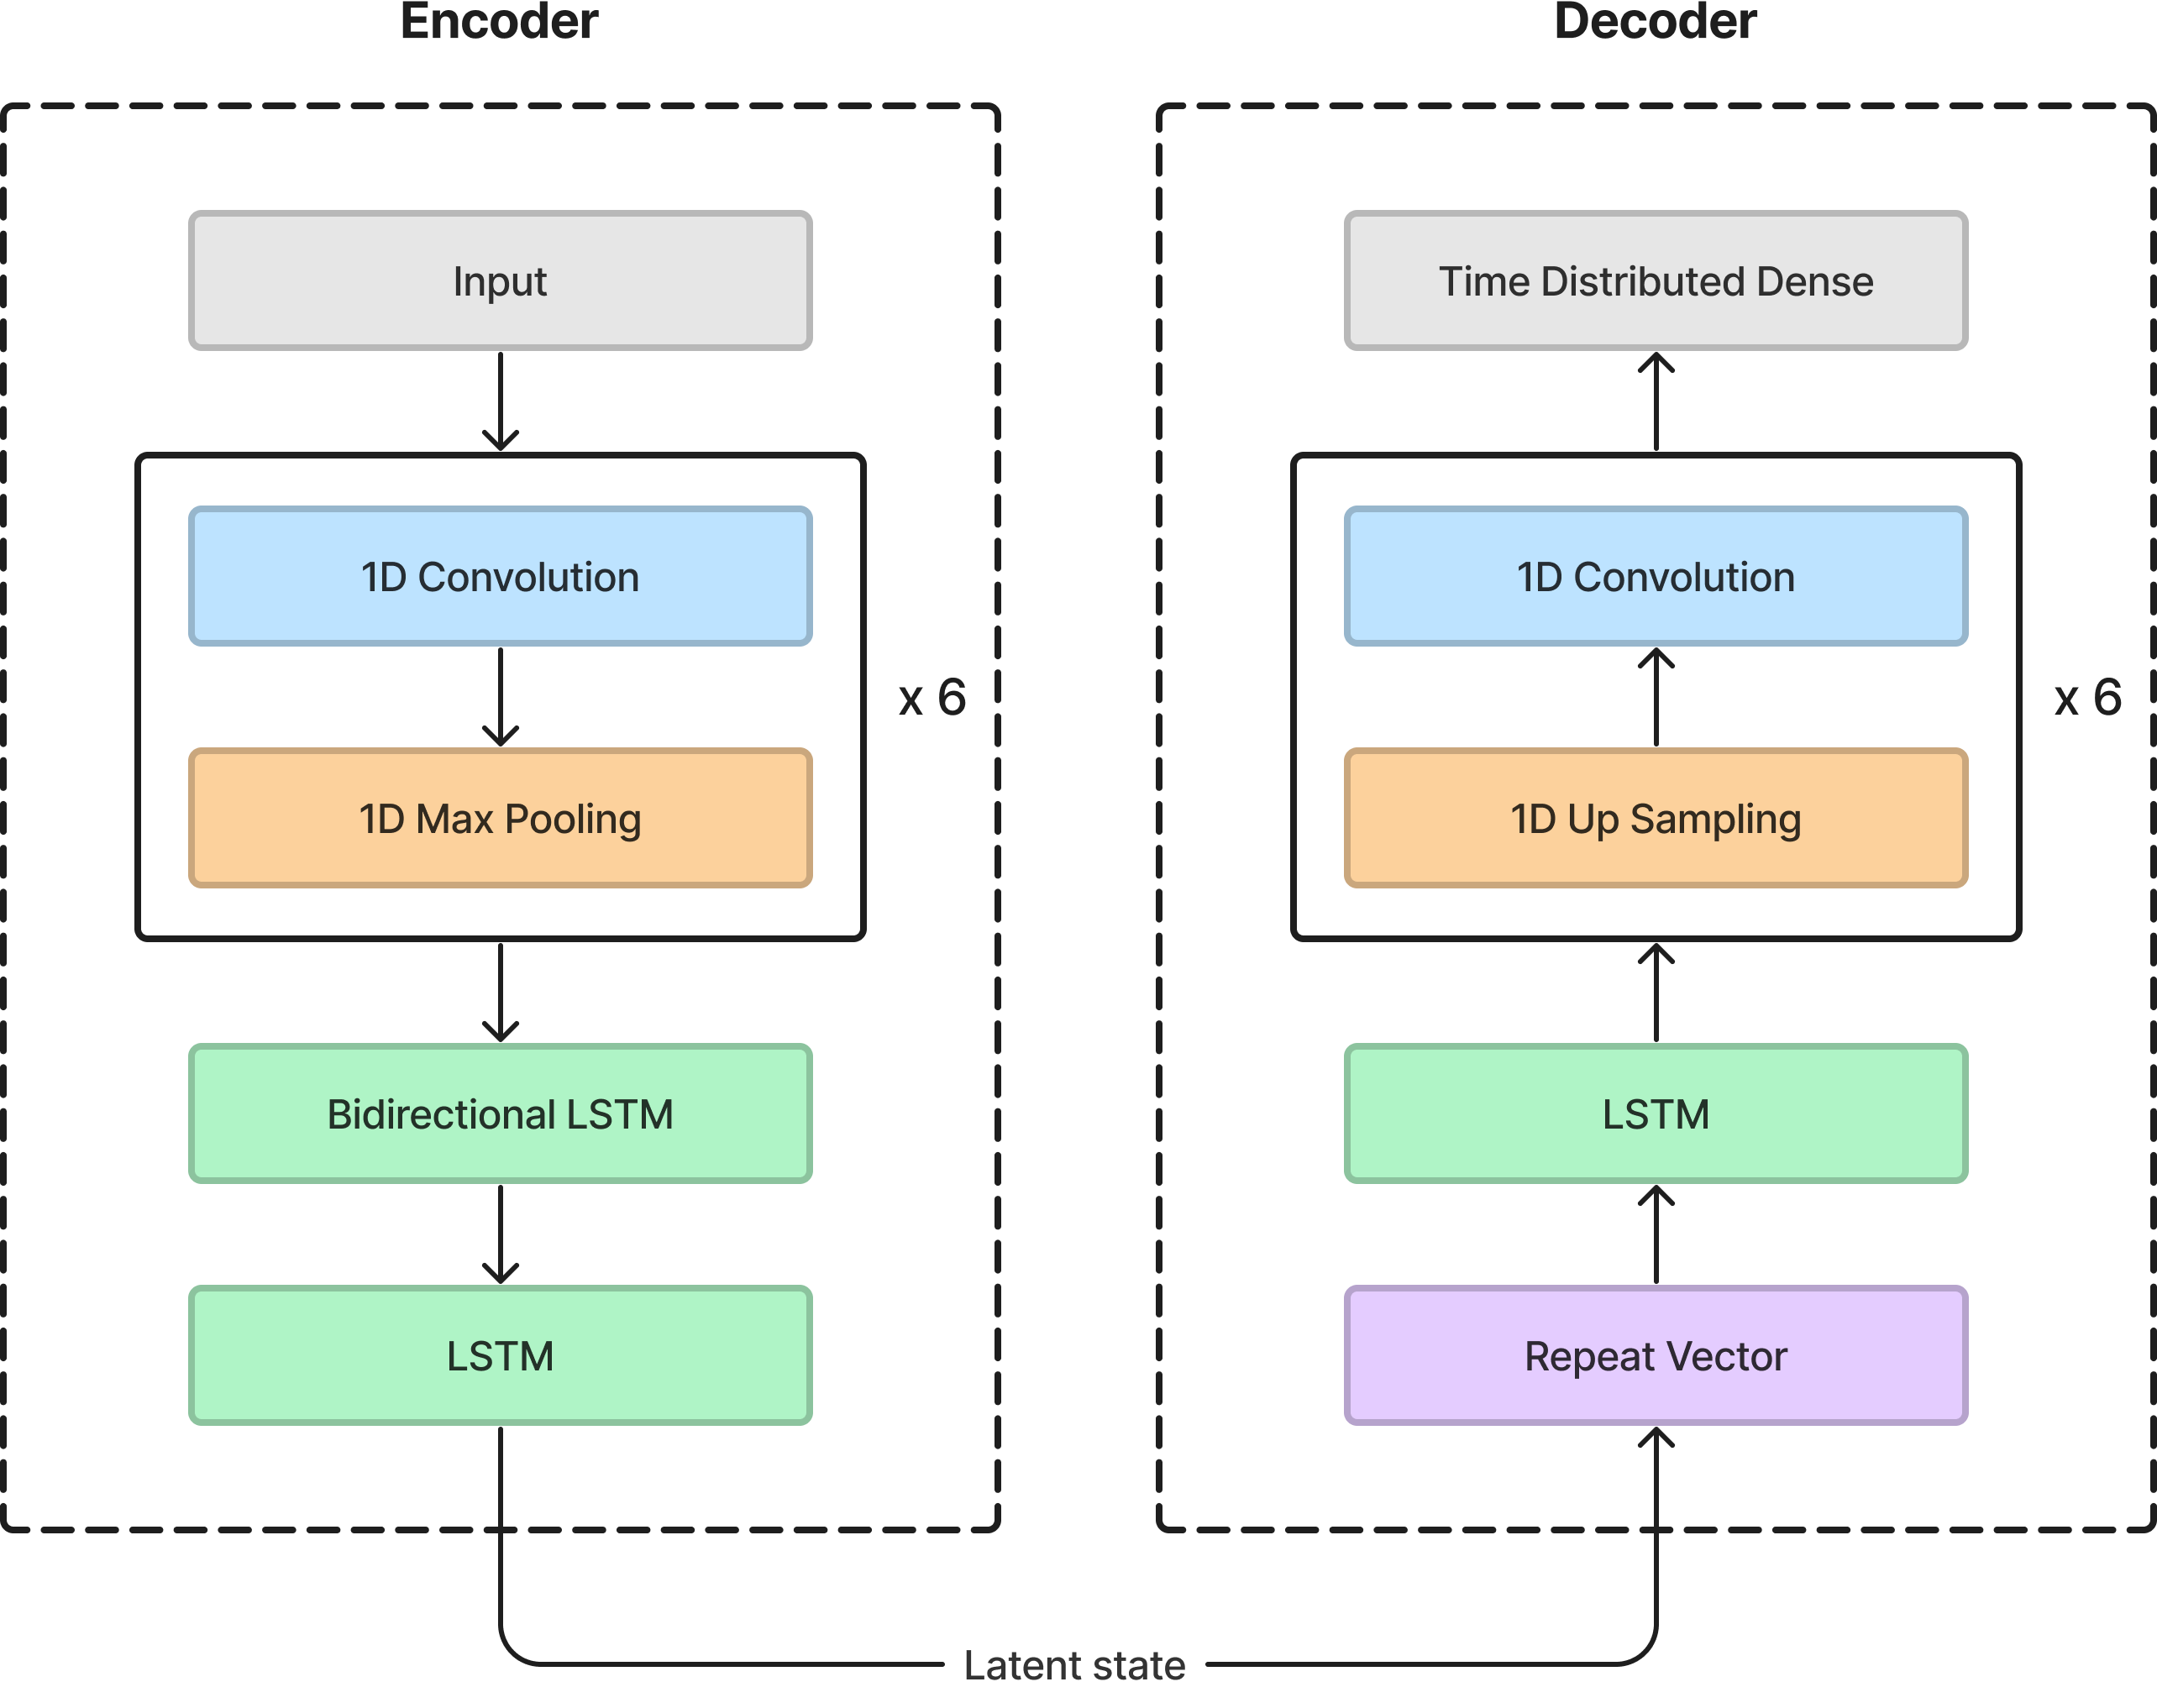
\includegraphics[width=.8\linewidth]{images/modes_clustering/autoencoder.png}
  \caption{Autoencoder architecture. The colors identify layers with similar purpose.}
  \label{fig:autoencoder_architecture}
\end{figure}

The model was implemented using Tensorflow~\parencite{abadiTensorFlowLargeScaleMachine2016,tensorflowdevelopersTensorFlow2023} version \texttt{2.15.0} and Keras~\parencite{cholletKeras2015}, in the version provided by Tensorflow. The Python version is \texttt{3.10.12}. The training was executed using a Google Colab notebook\footnote{\url{https://colab.research.google.com/drive/1blnoyyP10gGdRL6b4JzaeBLg8zs2kVv9?usp=sharing}}, running \texttt{Ubuntu 22.04.03 LTS} with the Linux kernel \texttt{6.1.58}, with an \texttt{Intel Xeon @ 2.00GHz} CPU, a \texttt{Tesla T4} GPU, and $12.6GB$ of RAM.

The loss function used is the mean square error between the output and the original input. The network parameters are optimized by using the \acrfull{adam} algorithm with a learning rate of $0.001$ and a batch size of $32$. The training process lasts for $500$ epochs at most, but it stops sooner if the loss value does not improve for $40$ epochs, returning the best model found. The $20\%$ of training instances were held out for training validation. All training instances are zero padded or truncated to $896$ samples. This number was chosen as it is close to the average length of all activations, and it is divisible by $2$ for $6$ times, which ensures that the up sampling layers in the decoder correctly reconstruct the input dimensions. The instances are then standardized using Equation~\eqref{equ:std}, where the mean $\mu_X$ and standard deviation $\sigma_X$ are computed across all the power measurements $X$. The evolution of the loss values during training are reported in Figure~\ref{fig:autoencoder_losses}.
\begin{equation}\label{equ:std}
  X_{scaled} = \frac{X - \mu_X}{\sigma_X}
\end{equation}

\begin{figure}
  \centering
  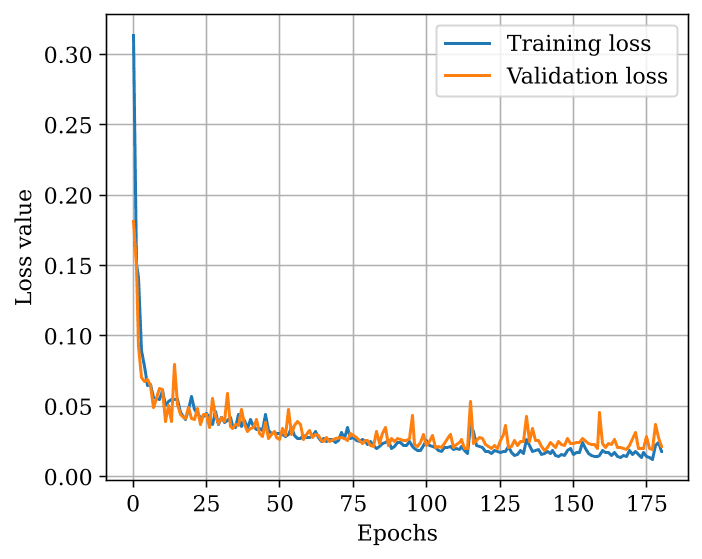
\includegraphics[width=.6\linewidth]{images/modes_clustering/loss.png}
  \caption{Evolution of training and validation losses during training.}
  \label{fig:autoencoder_losses}
\end{figure}

\section{Modes Clustering}

The complete clustering procedure for the operation modes of appliances is illustrated in Figure~\ref{fig:clustering}. First, the activations of each appliance are standardized using Equation~\eqref{equ:std}. Then, the latent state of each activation is obtained by applying the trained encoder. Next, the K-Means algorithm is used to cluster the latent states into $K$ groups. The algorithm iteratively assigns each latent state to the closest cluster centroid, calculated as the mean of all instances in a cluster, thus minimizing the mean squared distance between the instances and their centroids~\parencite{lloydLeastSquaresQuantization1982}. The algorithm converges when the centroids stop changing. The scikit-learn~\parencite*{pedregosaScikitlearnMachineLearning2011, buitinckAPIDesignMachine2013} implementation of K-Means was used, with the default settings that select a single initial centroid chosen by the \textit{k-means++} method, based on the points’ inertia. The algorithm also has a maximum of $300$ iterations and a tolerance of $0.0001$.

\begin{figure}
  \centering
  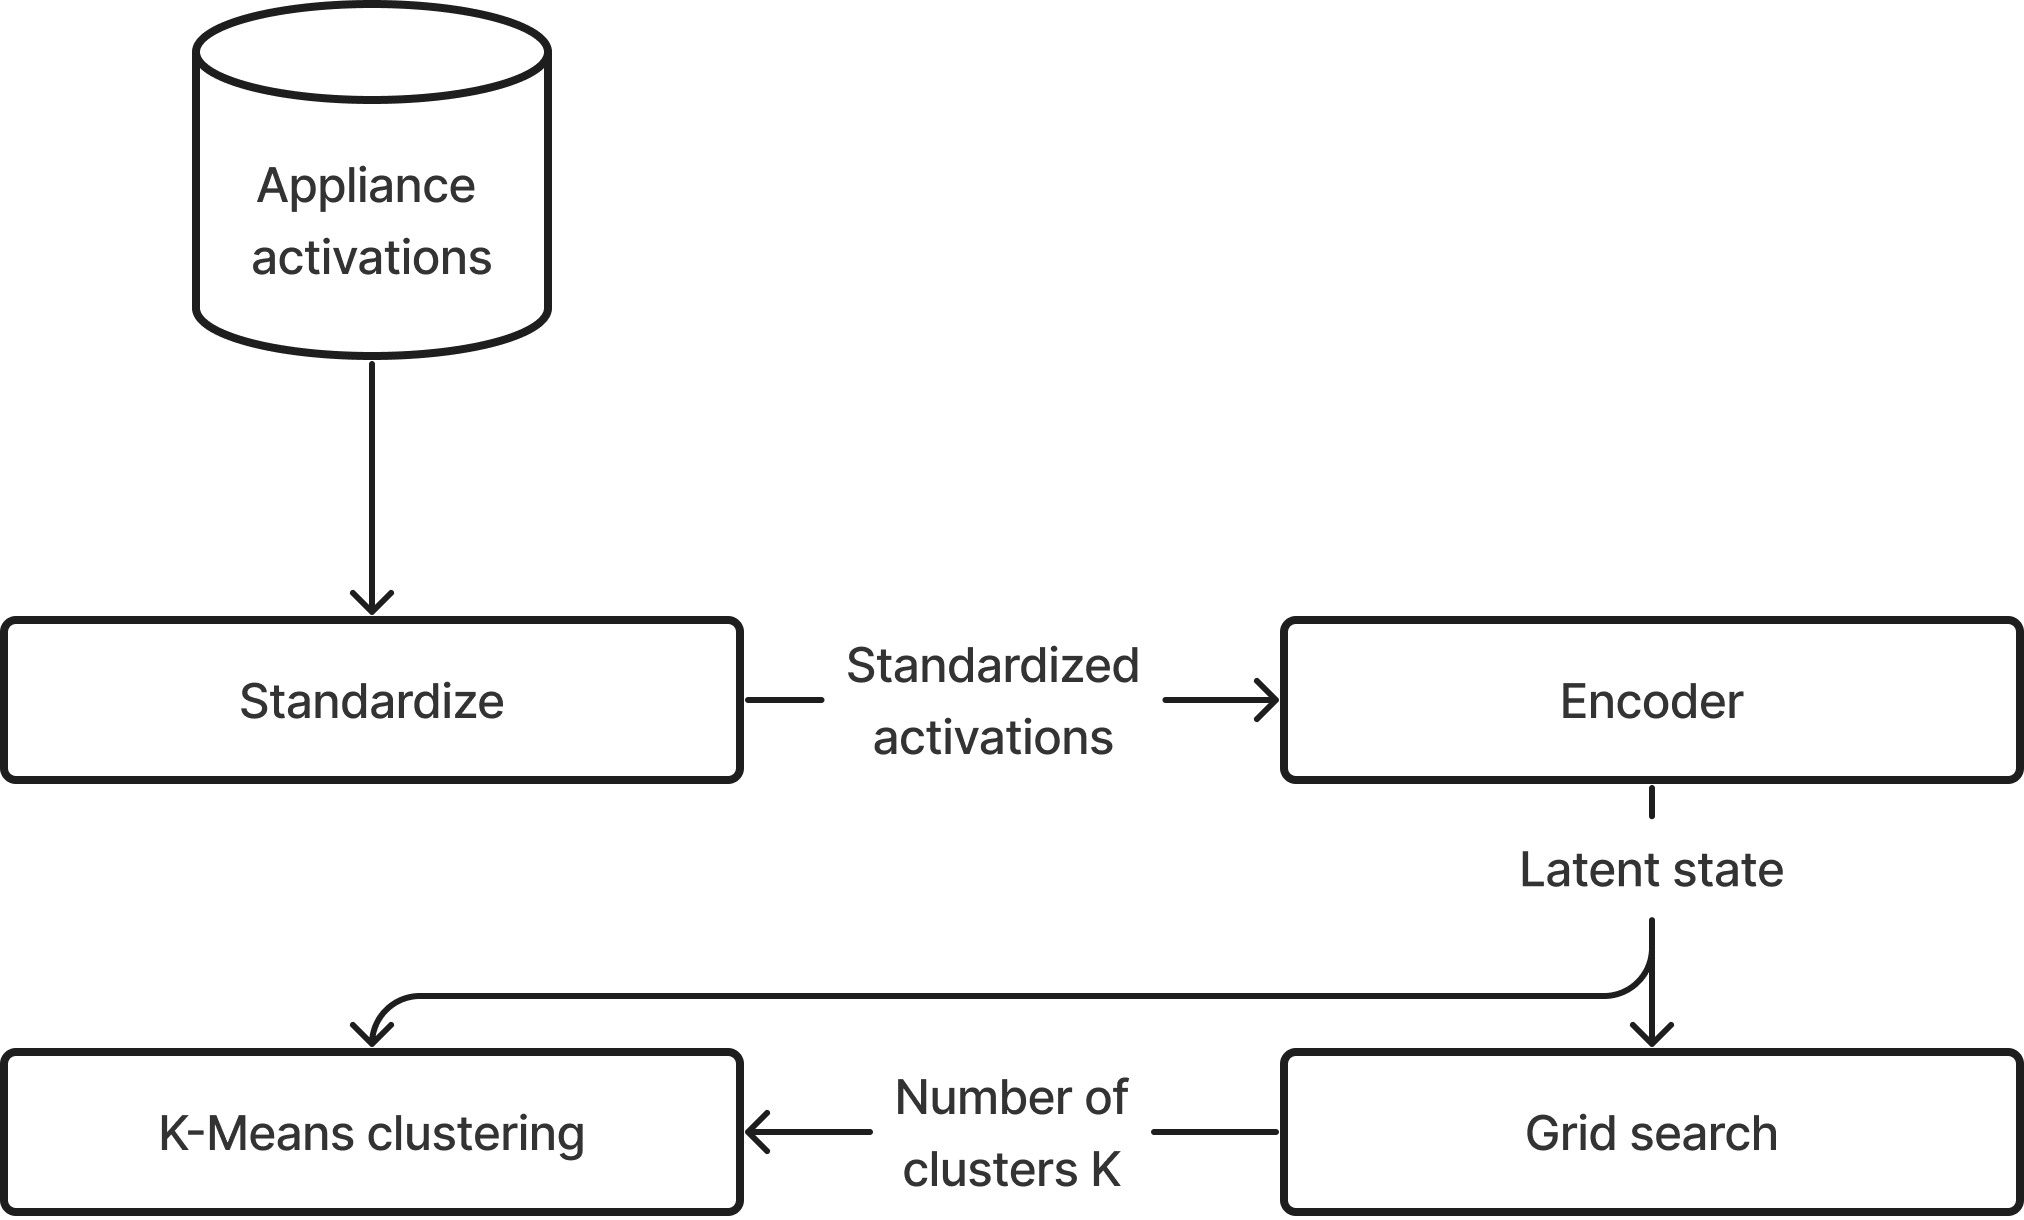
\includegraphics[width=.5\linewidth]{images/modes_clustering/clustering.png}
  \caption{Procedure for clustering the operation modes of appliances.}
  \label{fig:clustering}
\end{figure}

To find the optimal number of clusters K for each appliance, a grid search was run that evaluate the \textit{silhouette score} of each possible clustering. The silhouette score quantifies how well a latent state belongs to its cluster compared to other clusters~\parencite{rousseeuwSilhouettesGraphicalAid1987}. It is computed for each latent state using Equation~\eqref{equ:silhouette}, where $a(i)$ is the mean squared distance between the latent state and the other latent states in the same cluster, and $b(i)$ is the minimum mean squared distance between the latent state and the latent states in different clusters. The silhouette score ranges from $-1$ to $1$, with higher values indicating better clustering. The average silhouette score of all the latent states is used as a metric for the quality of the clustering as a whole.
\begin{equation}\label{equ:silhouette}
  s(i) = \frac{b(i) - a(i)}{\max{a(i), b(i)}}
\end{equation}

The clustering with the highest silhouette score was chosen. The search space for K was limited to values between $2$ and $4$, because lower values would not capture the diversity of the operation modes, and higher values would create too many noise clusters that could not be interpreted as meaningful modes. This also matches the realistic expectation that end users do not make use of all the operation modes for their appliances. For instance, it is possible that an end user only uses a washing machine for a few programs, such as a quick wash or a delicate wash, and never uses the other programs.

\section{Identification of Operation Modes}

The cluster labels were used to identify the operation modes of the appliance, and to estimate their duration. The procedure used for doing this is presented in Figure~\ref{fig:identification}.

\begin{figure}
  \centering
  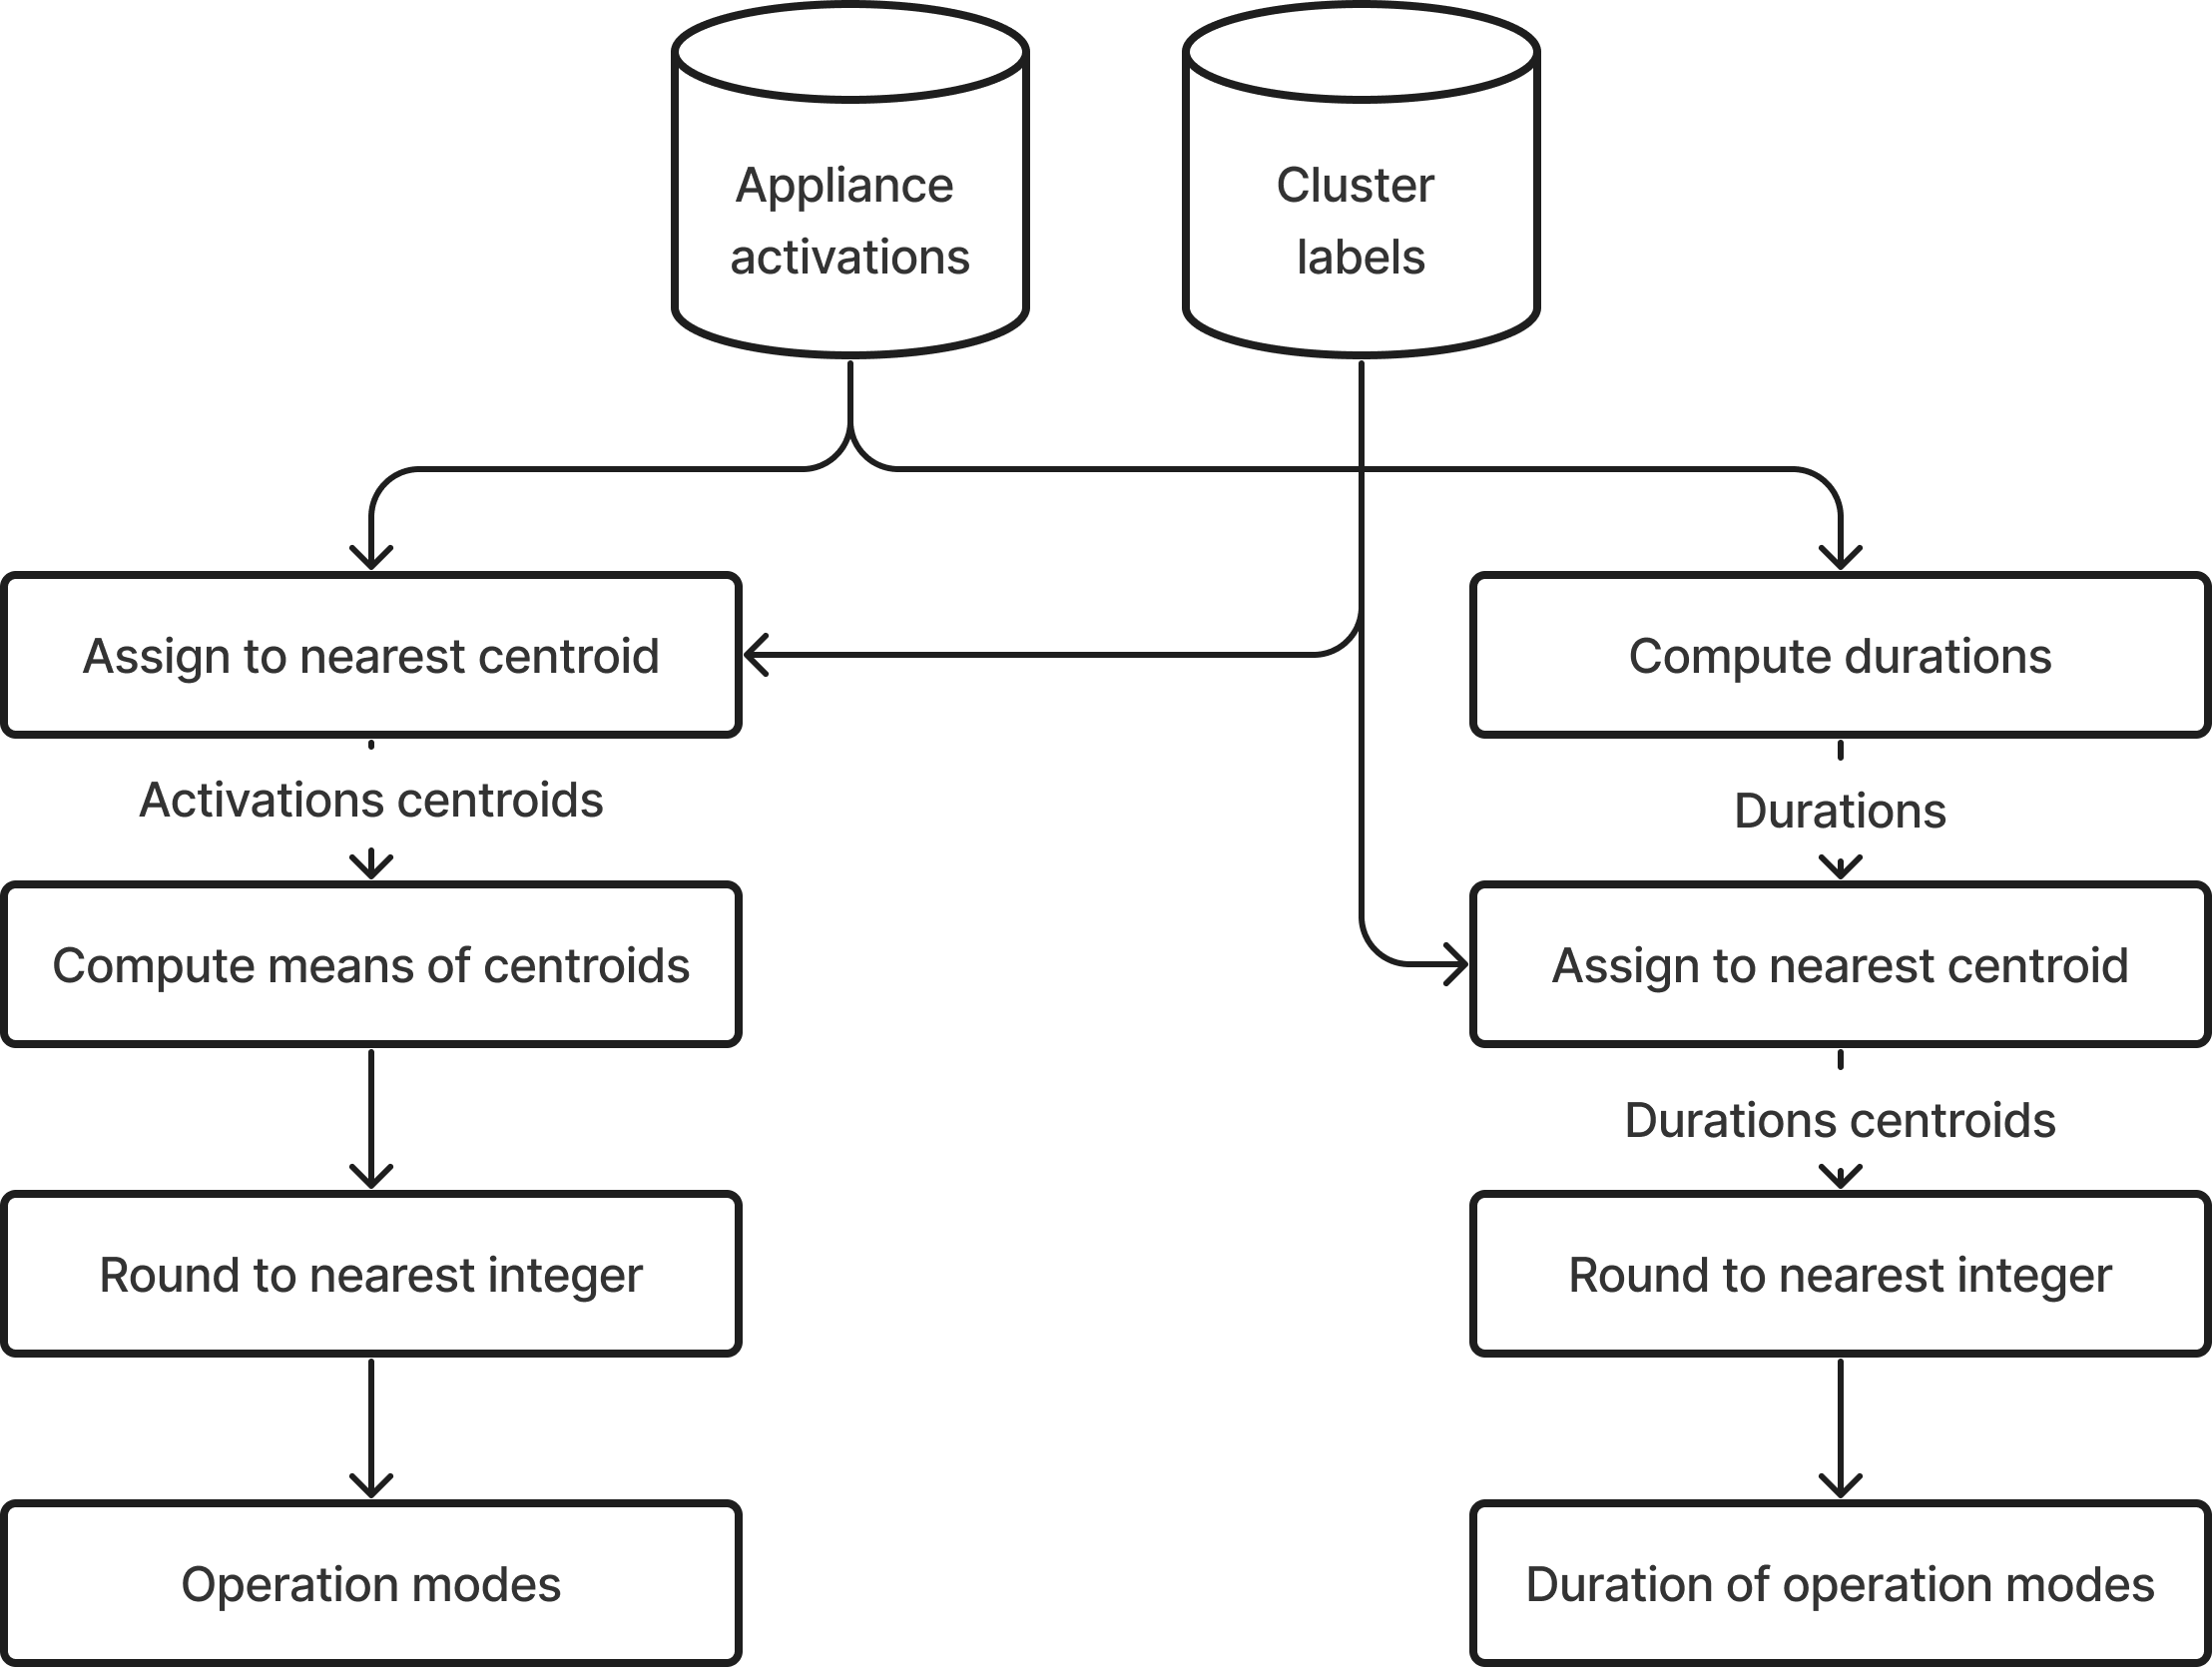
\includegraphics[width=.55\linewidth]{images/modes_clustering/identification.png}
  \caption{Procedure for clustering the operation modes of appliances.}
  \label{fig:identification}
\end{figure}

First, the appliance activations are assigned to the closest cluster centroid, which represents the mean activation of each cluster. Then, the mean power consumption value of each centroid is computed and rounded to the nearest integer. These values are the potential operation modes of the appliance. Next, a selection process is performed to merge or discard operation modes that have similar or unrealistic power consumption values, based on the device manuals. The manuals also provide the names for the identified modes. This procedure may not detect all the operation modes, especially if the end users do not use some of them frequently, or if the procedure confuses transitional states with modes.

Second, the duration of each operation mode is estimated by calculating the average duration (in seconds) of the activations that belong to the same cluster. The duration values are also rounded to the nearest integer. These values are used as default durations for the operation modes. These preliminary results obtained are reported in Table~\ref{tab:preliminary_identification_results}.

\begin{table}[hbt]
  \centering
  \resizebox{.39\textwidth}{!}{%
    \begin{tblr}{llcc}
      \hline
      \textbf{Appliance type}             & \textbf{Consumption (W)} & \textbf{Duration (s)} \\ \hline
      \SetCell[r=2]{l}{Radio}             & 1                        & 80                    \\
                                          & 37                       & 4435                  \\ \hline[dashed]
      \SetCell[r=4]{l}{Dishwasher}        & 136                      & 2359                  \\
                                          & 12                       & 240                   \\
                                          & 54                       & 3025                  \\
                                          & 41                       & 459                   \\ \hline[dashed]
      \SetCell[r=2]{l}{Fridge w/ freezer} & 208                      & 6304                  \\
                                          & 7                        & 37                    \\ \hline[dashed]
      \SetCell[r=2]{l}{Television}        & 18                       & 2514                  \\
                                          & 110                      & 1833                  \\ \hline[dashed]
      \SetCell[r=2]{l}{Microwave}         & 42                       & 302                   \\
                                          & 1265                     & 1433                  \\ \hline[dashed]
      \SetCell[r=2]{l}{Lamp}              & 2                        & 309                   \\
                                          & 19                       & 587                   \\ \hline[dashed]
      \SetCell[r=4]{l}{Washing machine}   & 82                       & 1176                  \\
                                          & 118                      & 1486                  \\
                                          & 1281                     & 1309                  \\
                                          & 1783                     & 1511                  \\ \hline[dashed]
      \SetCell[r=2]{l}{Desktop}           & 4                        & 1159                  \\
                                          & 41                       & 12412                 \\ \hline[dashed]
      \SetCell[r=3]{l}{Boiler}            & 33                       & 300                   \\
                                          & 57                       & 525                   \\
                                          & 101                      & 2187                  \\ \hline[dashed]
      \SetCell[r=3]{l}{AC}                & 71                       & 199                   \\
                                          & 336                      & 3337                  \\
                                          & 656                      & 30176                 \\ \hline
    \end{tblr}%
  }
  \caption[Preliminary results of operation modes identification]{Preliminary results of operation modes identification. The \textit{off} mode is not reported, as it is assumed to have 0W consumption and indeterminate duration for all appliances.}
  \label{tab:preliminary_identification_results}
\end{table}

The procedure works well for simple appliances, such as the lamp or the television, whose operation modes are easy to distinguish. However, it has some limitations for more complex appliances, such as the washing machine, the dishwasher, and the microwave. For these appliances, the procedure fails to identify the correct operation modes and their durations, due to the following reasons:
\begin{itemize}
  \item The sequence length of $896$ is too short to capture the full cycle of these appliances, which may have multiple operation modes in one activation.
  \item The number of training instances for the autoencoder is too small to learn the features of these appliances, which may have high variability in their activations.
  \item The extraction of the activations is based on an empirical threshold, which may not be optimal for these appliances, whose power consumption may fluctuate or overlap with other appliances.
  \item The operation modes are too similar to each other, or there are too many to be distinguishable. This could be the case of the microwave, which allows the user to manually configure the power level of each operation mode, thus creating a large number of possibilities.
\end{itemize}

Therefore, for the washing machine, dishwasher, and microwave, the operation modes and their durations were extracted from the manuals of the devices. For appliances with configurable operation modes, only a single configuration was chosen to represent each mode. The identified durations for \textit{stand-by} or \textit{suspended} operation modes were set to $\infty$, as such modes tipically remain active until the user explicitly changes them. Table~\ref{tab:identification_results} summarizes the results of the identification procedure for all the appliances.

\begin{table}
  \centering
  \resizebox{.6\textwidth}{!}{%
    \begin{tblr}{llcc}
      \hline
      \textbf{Appliance type}           & \textbf{Mode name} & \textbf{Consumption (W)} & \textbf{Duration (s)} \\ \hline
      \SetCell[r=2]{l}{Radio}           & Stand-by           & 1                        & $\infty$              \\
                                        & On                 & 37                       & 4435                  \\ \hline[dashed]
      \SetCell[r=6]{l}{Dishwasher}      & Intensive          & 1400                     & 10380                 \\
                                        & Daily              & 810                      & 10260                 \\
                                        & Eco                & 700                      & 6660                  \\
                                        & Express            & 350                      & 1680                  \\
                                        & Delicate           & 800                      & 7080                  \\
                                        & Pre-wash           & 10                       & 660                   \\ \hline[dashed]
      Fridge w/ freezer                 & On                 & 208                      & 6304                  \\ \hline[dashed]
      \SetCell[r=2]{l}{Television}      & Stand-by           & 18                       & 2514                  \\
                                        & On                 & 110                      & 1833                  \\ \hline[dashed]
      \SetCell[r=7]{l}{Microwave}       & Stand-by           & 5                        & $\infty$              \\
                                        & Microwave          & 750                      & 300                   \\
                                        & Crisp              & 500                      & 300                   \\
                                        & Grill              & 500                      & 300                   \\
                                        & Grill+microwave    & 500                      & 300                   \\
                                        & Steam              & 350                      & 300                   \\
                                        & Jet defrost        & 160                      & 300                   \\ \hline[dashed]
      Lamp                              & On                 & 19                       & 587                   \\ \hline[dashed]
      \SetCell[r=7]{l}{Washing machine} & Cotton 90°         & 2000                     & 8700                  \\
                                        & Cotton 60E         & 950                      & 7680                  \\
                                        & Cotton 60°         & 1200                     & 7200                  \\
                                        & Cotton 30°         & 550                      & 6900                  \\
                                        & Synthetic 30°      & 900                      & 5400                  \\
                                        & Delicate 30°       & 500                      & 3600                  \\
                                        & Wool               & 450                      & 3300                  \\ \hline[dashed]
      \SetCell[r=2]{l}{Desktop}         & Suspended          & 4                        & $\infty$              \\
                                        & On                 & 41                       & 12412                 \\ \hline[dashed]
      \SetCell[r=3]{l}{Boiler}          & Holiday            & 33                       & 300                   \\
                                        & Comfort            & 57                       & 525                   \\
                                        & Auto               & 101                      & 2187                  \\ \hline[dashed]
      \SetCell[r=2]{l}{AC}              & Cool               & 336                      & 3337                  \\
                                        & Heat               & 656                      & 30176                 \\ \hline
    \end{tblr}%
  }
  \caption[Results of operation modes identification]{Results of operation modes identification. The \textit{off} mode is not reported, as it is assumed to have 0W consumption and indeterminate duration for all appliances.}
  \label{tab:identification_results}
\end{table}
